%%%%%%%%%%%%%%%%%%%%%%%%%%%%%%%%%%%%%%%%%%%%%%%%%%%%%%%%%%
\section{Using Biases}
%%%%%%%%%%%%%%%%%%%%%%%%%%%%%%%%%%%%%%%%%%%%%%%%%%%%%%%%%%

This section make use of the new central bias model (similar to \cite{clarke-tatler2014} expect uses a truncated Gaussian distrubition to take the image boundaries into accout) and the \textit{saccadic flow} model (described in \ref{ModellingFlow}). We present two examples of how these bias models can be used as a prior in order to weight fixations. First of all, we will demonstrate how we can weight fixations in hotspot maps to reduce the noise and give an improved visualisation of the regions of the image that participants looked at more than expect. Secondly, we will demonstrate how these priors can be used in ROC analysis to improve results. We will re-analyse the effect of the scene context model developed by  \cite{ehinger2009} as an example. 

\subsection{Gaze landscapes}

One technique that is commonly used to visualise the spatial allocation of gaze is to create 'heatmap' plots where colour or luminance are used to indicate the density of fixation on those locations (Figure ~\ref{fig:adjustedHeatmaps}, column 2). Some argue that one problem with visualising data in this way is that they represent all fixations as equal. For example, a fixated location with a fixation of a second would be weighted equally with fixations that lasted half that time. If we want to make an assumption that fixation duration is intimately linked with the importance of that fixation (i.e. we will look longer at more informative information) then we can change our visualisation to weight fixations by their duration (Figure ~\ref{fig:adjustedHeatmaps}, column 3).

One advantage of the \citep{clarke-tatler2014} model, and the saccadic flow model here is that we can represent fixations by the likelihood that they would occur based on the predictions of the models. As there is an image independent tendency to fixate in the centre of the scene (for example), then we might consider that saccades to locations less predicted by these behavioural and oculomotor biases might involve more high-level mechanisms. In Figure ~\ref{fig:adjustedHeatmaps} (column 4 and 5) we present some overlaid heatmap data from the \citep{clarke2013} dataset, where fixations are weighted by the inverse probability of them occuring based on the models of central bias and saccadic flow. These figures reveal that representing data in this manner can allow us to visualise information that was important enough to break the biases of looking at the scene centre, or making saccades in line with our saccadic flow model. We can therefore use this to remove some of the image-independent biases, and reveal the more important image \emph{dependent} information.

\begin{figure*}
\includegraphics[width=\textwidth]{figs/adjustedheatmaps.pdf}
\caption{Traditional 'heat map' plots of fixations normalised by the central bias. This method allows us to characterise fixations that are less accountable for by image-independent central biases.}
\label{fig:adjustedHeatmaps}
\end{figure*}

Or do we call them hotspot maps?

\subsection{Reanalysis of Clarke et al 2013}

Do the flow-weights offer an improvement on predicting named objects over the fixations-weights?

\subsection{Reanalysis of Ehinger et al 2009}

Re-analysis of \cite{ehinger2009} comparing ROC methods for leave-one-out, uniform, central bias and flow. How well does their context model work in each test>

\subsection{Comparison between synthetic and real data}

To what extent does saccadic flow account for coarse-to-fine dynamics? Not that well. Not unexpected.

We can see from Figure \ref{fig:xyDist} that both the central bias and the saccadic flow model do an good job of capturing the distribution of fixation locations in the $x$ and $y$ axes. However, the saccades generated by the flow model tend to be slightly larger than those made by human observers (Figure \ref{fig:saccAmp}). 

\begin{figure*}[htb]
\centering
\subfigure{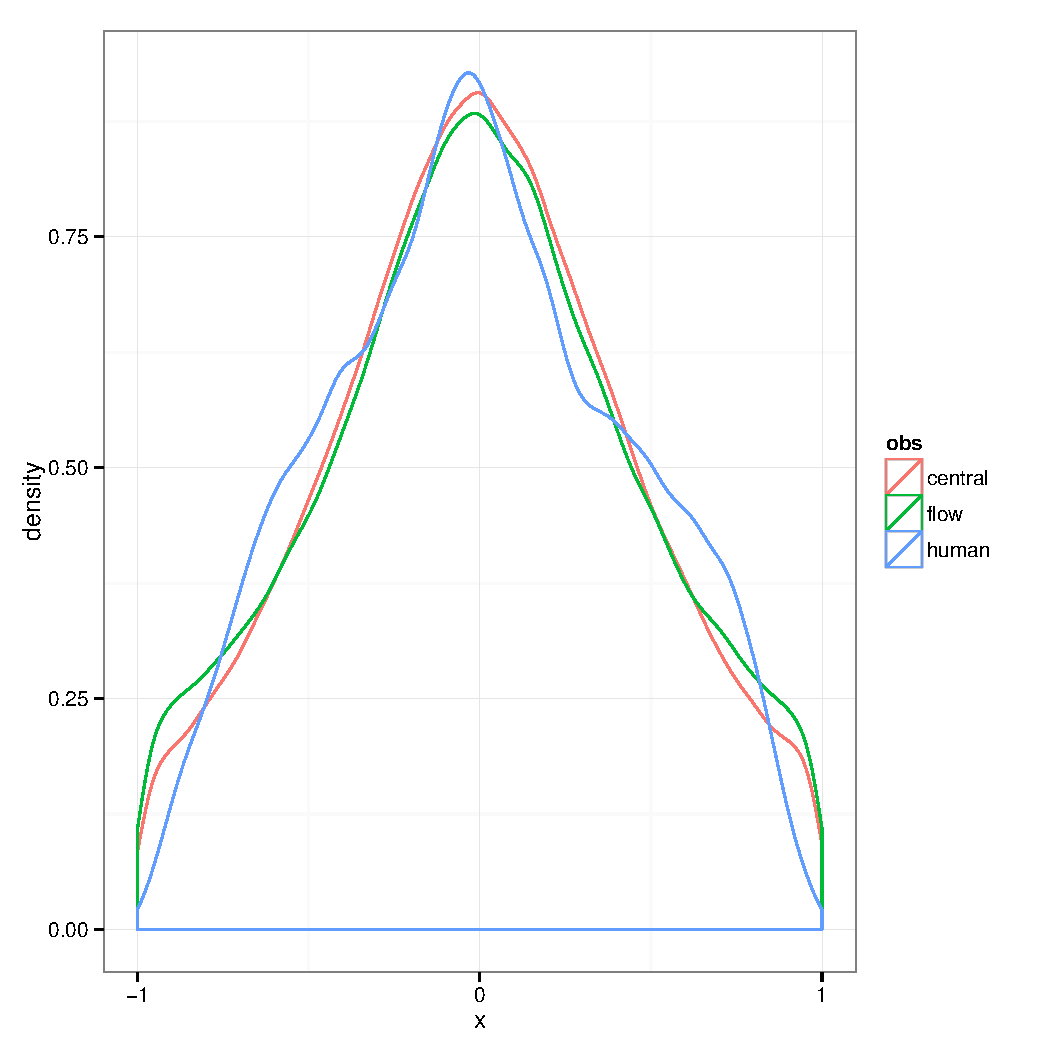
\includegraphics[width=6cm]{../scripts/coarse2fine/figs/xFixComparison}}
\subfigure{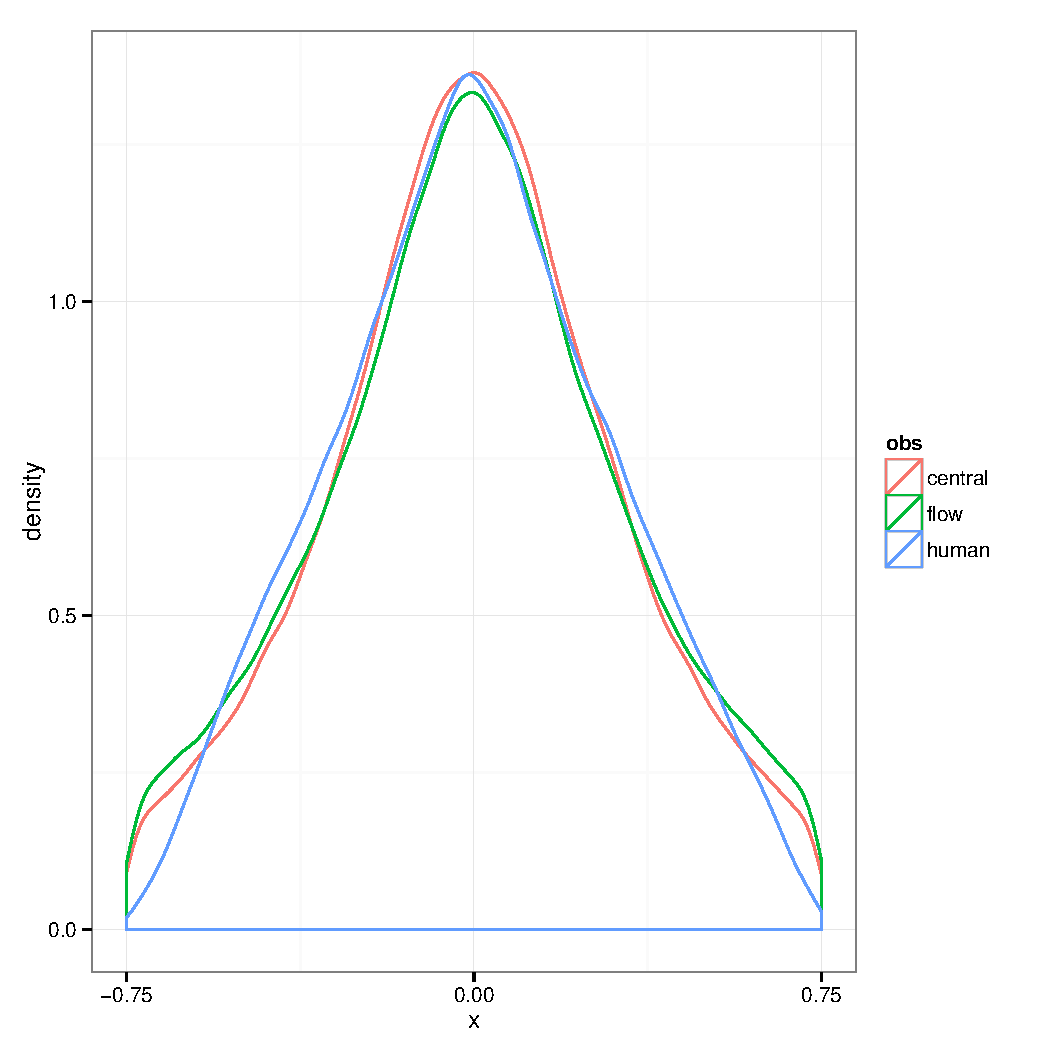
\includegraphics[width=6cm]{../scripts/coarse2fine/figs/yFixComparison}}
\caption{Comparison of $x$ and $y$ fixation positions between human fixations and synthetic points generated from the central bias and flow model. Note, using tN central bias.}
\label{fig:xyDist}
\end{figure*}

\begin{figure*}[htb]
\centering
\subfigure{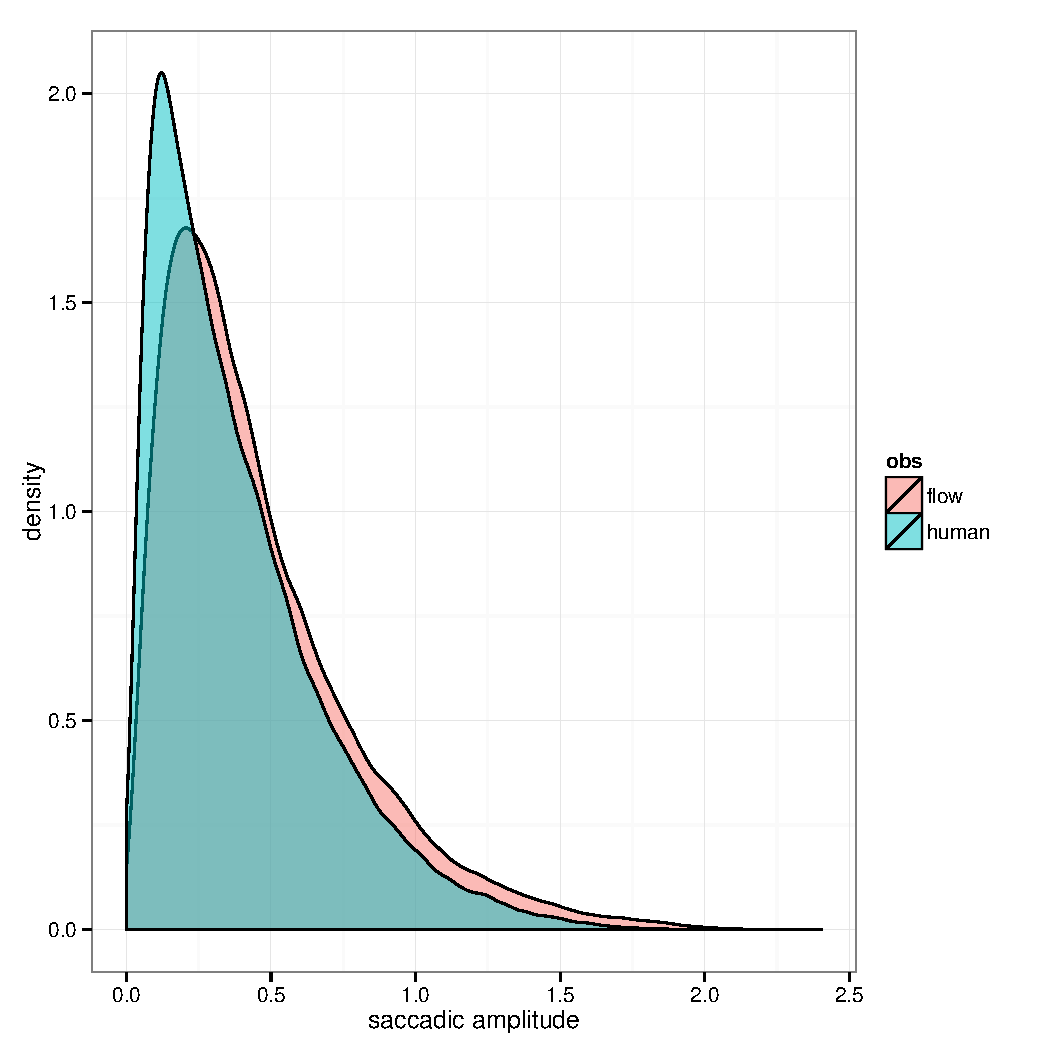
\includegraphics[width=6cm]{../scripts/coarse2fine/figs/ampSaccComparison}}
\subfigure{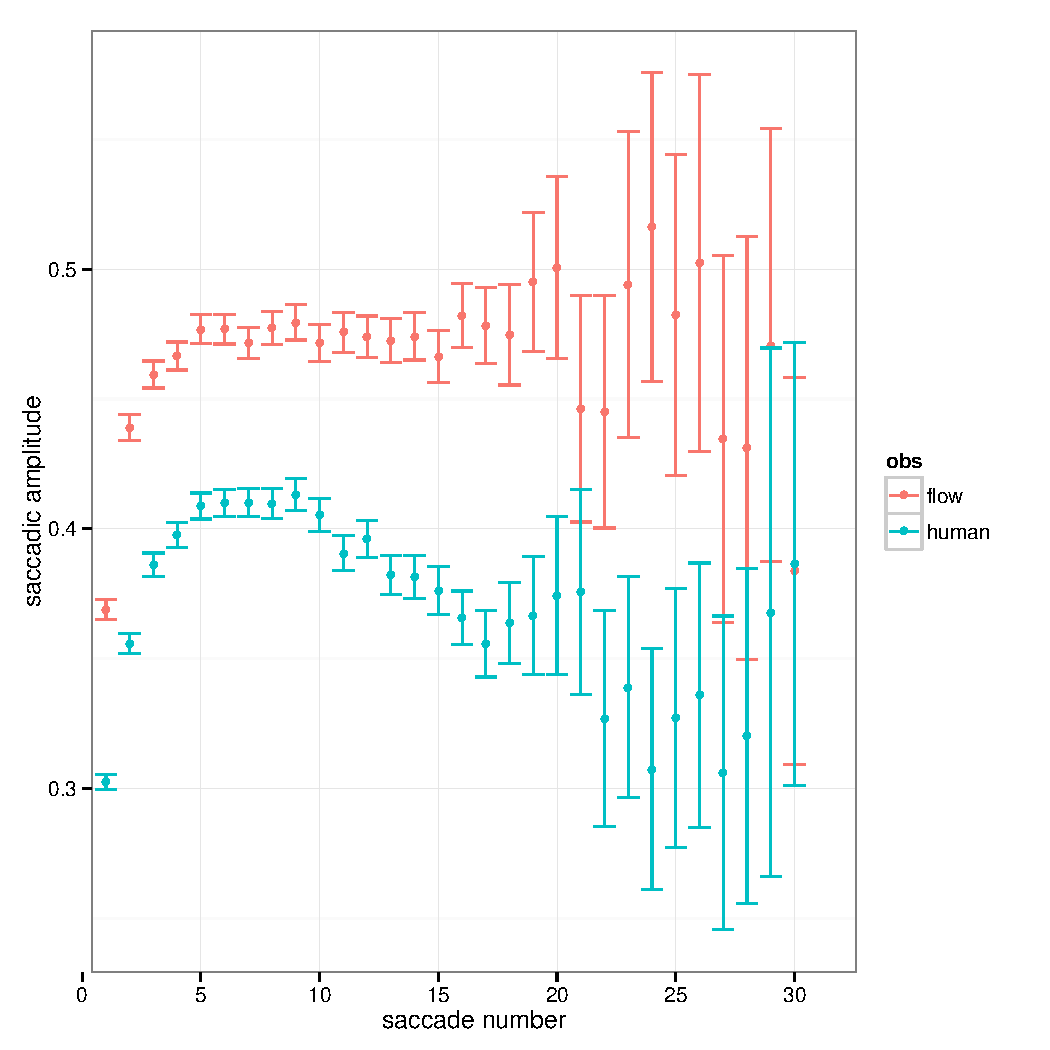
\includegraphics[width=6cm]{../scripts/coarse2fine/figs/saccAmpOverTimeFlow}}
\caption{We can see that the flow model consistently makes saccades with a slightly larger amplitude than human observers.}
\label{fig:saccAmp}
\end{figure*}

